% !TeX root = ../main.tex
% !TeX root = ../main.tex
% Add the above to each chapter to make compiling the PDF easier in some editors.

\chapter{Optimization and Alternative Technologies}\label{chapter:optimization_and_alternative_technologies}

This chapter presents an insight into collected log and error metrics, a detailed analysis of the performance of GoCast's Workers, as well as an optimization approach for the main GoCast\ac{API} that compares the current REST \ac{API} with a prototype of a gRPC \ac{API}.   

\section{Monitoring Stack}

The GoCast system uses a rather complex stack of monitoring, logging, and analytics tools to collect metrics. The main technologies include \href{https://github.com/grafana/grafana}{Grafana}, \href{https://github.com/prometheus/prometheus}{Prometheus}, \href{https://github.com/influxdata/telegraf}{Telegraf}, and \href{https://github.com/influxdata/influxdb}{InfluxDB}, which are deployed in a containerized environment using Docker and managed by \href{https://github.com/traefik/traefik}{Traefik} as a reverse proxy. The collected data is then organized into Grafana dashboards. The metrics collection and logging system for TUMLive is based on the following main components:
\begin{itemize}
    \item \textbf{\href{https://github.com/grafana/grafana}{Grafana}}: This is used as the main dashboard for visualizing metrics and performance logs. It connects to various data sources, such as InfluxDB, for real-time monitoring of services.
    \item \textbf{\href{https://github.com/prometheus/prometheus}{Prometheus}}: As a monitoring and alerting toolkit, Prometheus is responsible for scraping metrics from the various services within the system.
    \item \textbf{\href{https://github.com/influxdata/telegraf}{Telegraf}}: This service collects metrics and logs from Docker containers, the host system, and various applications. It works together with InfluxDB to store time-series data.
    \item \textbf{\href{https://github.com/influxdata/influxdb}{InfluxDB}}: A time-series database, InfluxDB is utilized for storing logs and metrics collected from Telegraf, which are then visualized through Grafana.
    \item \textbf{\href{https://github.com/grafana/loki}{Loki}} and \textbf{\href{https://grafana.com/docs/loki/latest/send-data/promtail/}{Promtail}}: These tools are used for centralized logging, allowing for real-time querying and log analysis through Grafana's Loki integration.
    \item \textbf{\href{https://mariadb.org/}{MariaDB}}: Used as the primary database for storing TUMLive application data and internal user stats (see \autoref{subsection:user-stats-tumlive}).
\end{itemize}

\section{Metrics of the GoCast API}

The main data source for the GoCast \ac{API} were Loki and Traefik as well as internal server logs. This section will give some insights on common errors and patterns found in the main \ac{API} and (given the limited amount of logging data) focus on two main aspects: The number of errors and the observed errors types. The Python scripts for the plots for this and the following sections be found at \href{https://github.com/carlobortolan/Thesis/tree/analytics}{github.com/carlobortolan/thesis/analytics}.

\subsection{Error Volume Analysis}

Plotting the logged errors of the \ac{API} over time (see \autoref{fig:api-cum-errors-over-time}) shows an increase in the sum of total \ac{API} errors with a constant, positive slope. This indicates that errors were being logged at a relatively similar rate throughout the observed period. The fact that there are no obvious sudden spikes or drops in this data suggests a continuous, recurring issue rather than isolated incidents. Since the slope did not flatten over time, it shows that the error volume did not escalate or improve significantly over time, implying that either no major fixes were implemented to resolve the underlying causes during this time frame or new bugs were introduced with prior fixes.

\begin{figure}[htpb]
    \centering
    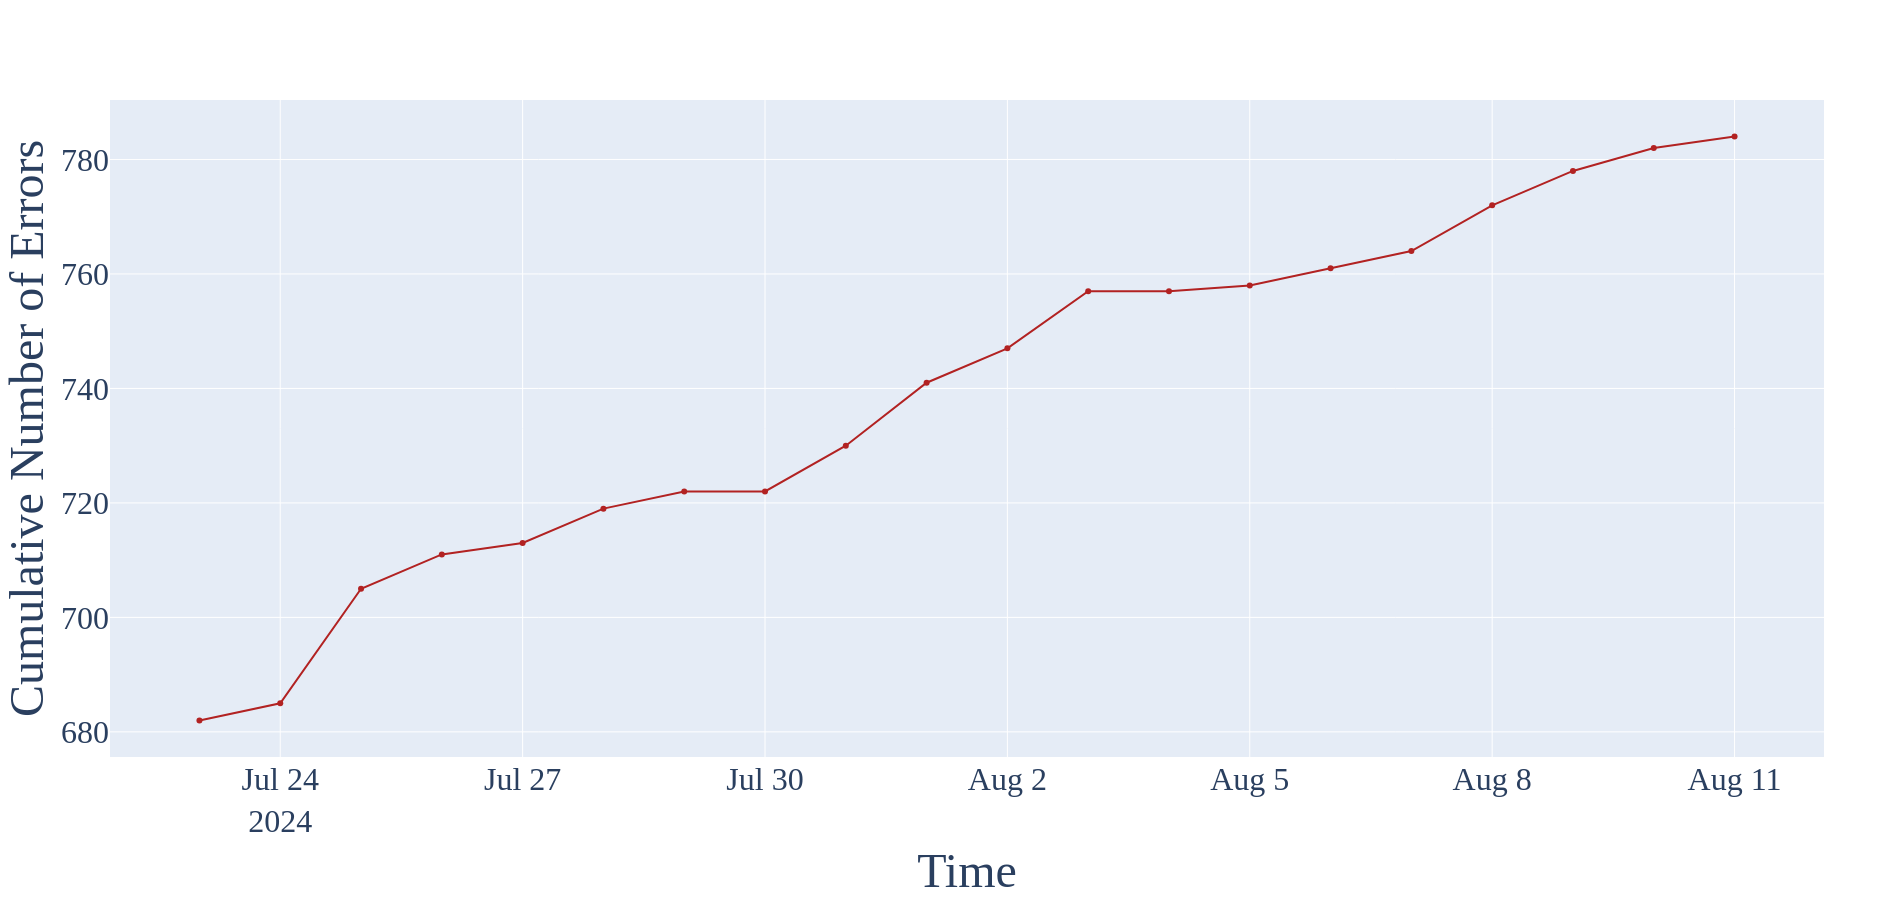
\includegraphics[width=\linewidth]{images/plots/api/cum_errors_over_time.png}
    \caption[Cumulative \ac{API} Errors Over Time]{Cumulative \ac{API} Errors Over Time}\label{fig:api-cum-errors-over-time}
\end{figure}

% \begin{figure}[htpb]
%     \centering
%     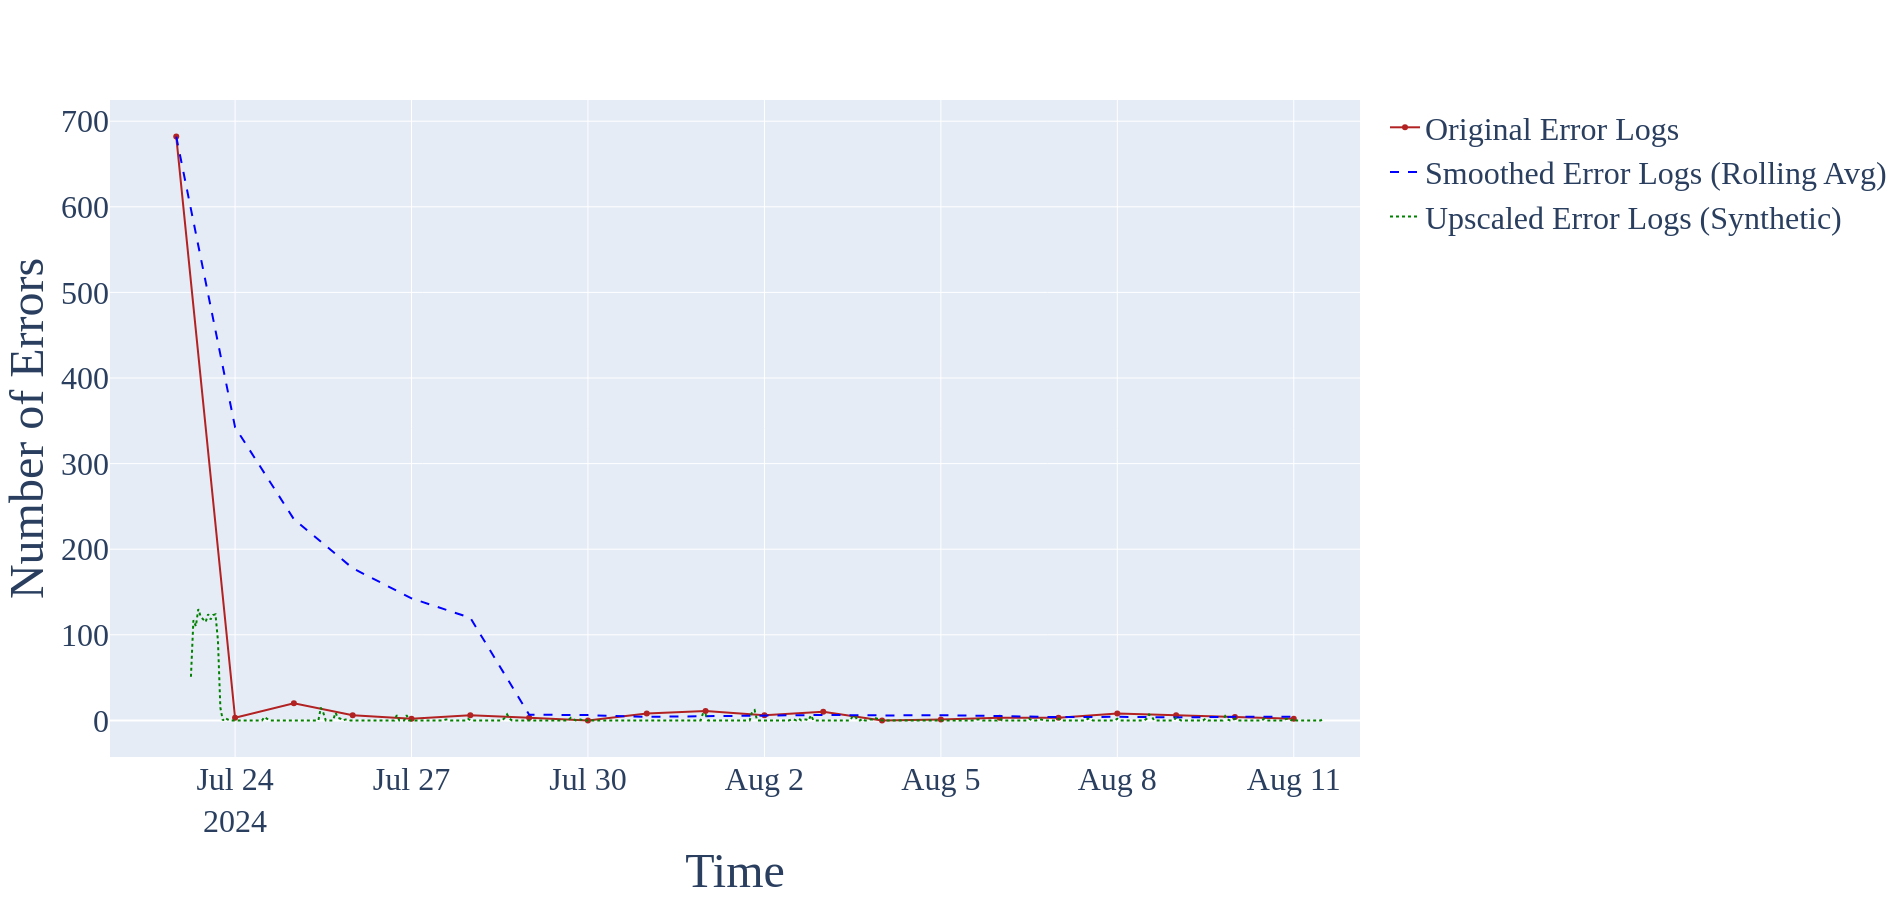
\includegraphics[width=\linewidth]{images/plots/api/upscaled_error_logs.png}
%     \caption[Upscaled \ac{API} Error Logs]{Upscaled \ac{API} Error Logs}\label{fig:api-upscaled-error-logs}
% \end{figure}

\subsection{Categorization of Error Types}

The errors aren't logged with a specific error type, but they contain a JSON String from which one can infer the origin of the error (e.g., see \autoref{fig:api-error-json}).

\begin{figure}[htpb]
  \begin{tabular}{c}
  \ \small \begin{lstlisting}[language=Java]
    {
      "time": "2024-07-23T06:38:08.282288184+02:00",
      "level": "ERROR",
      "msg": "Could not generate live preview",
      "service": "api",
      "err": "rpc error: code = Unknown desc = exit status 1"
    }
    \end{lstlisting}
  \end{tabular}
  \caption[Example API Error JSON]{Example API Error JSON}\label{fig:api-error-json}
\end{figure}

As seen in \autoref{fig:api-error-types}, the most common error logged by the \ac{API} was \textit{'Could not generate live preview'} with 677 occurrences. To understand this error, first it is necessary to explain that GoCast allows admins to trigger certain cron jobs which then periodically perform a certain action such as importing courses from CAMPUSonline, or in this case - fetching the thumbnails of livestreams (Live Previews) from the GoCast Workers. Hence, this error is a result of the \texttt{FetchLivePreviews} cron job which is performed every minute to get a live thumbnail from a worker. If this request returns an error, it logs the  ends the connection and decrements the worker's workload. Possible reasons for this could be network issues preventing the communication with the Worker, general Worker unavailability, or invalid or incomplete parameters passed to the \texttt{getLivePreviewFromWorker} function.

\begin{figure}[htpb]
    \centering
    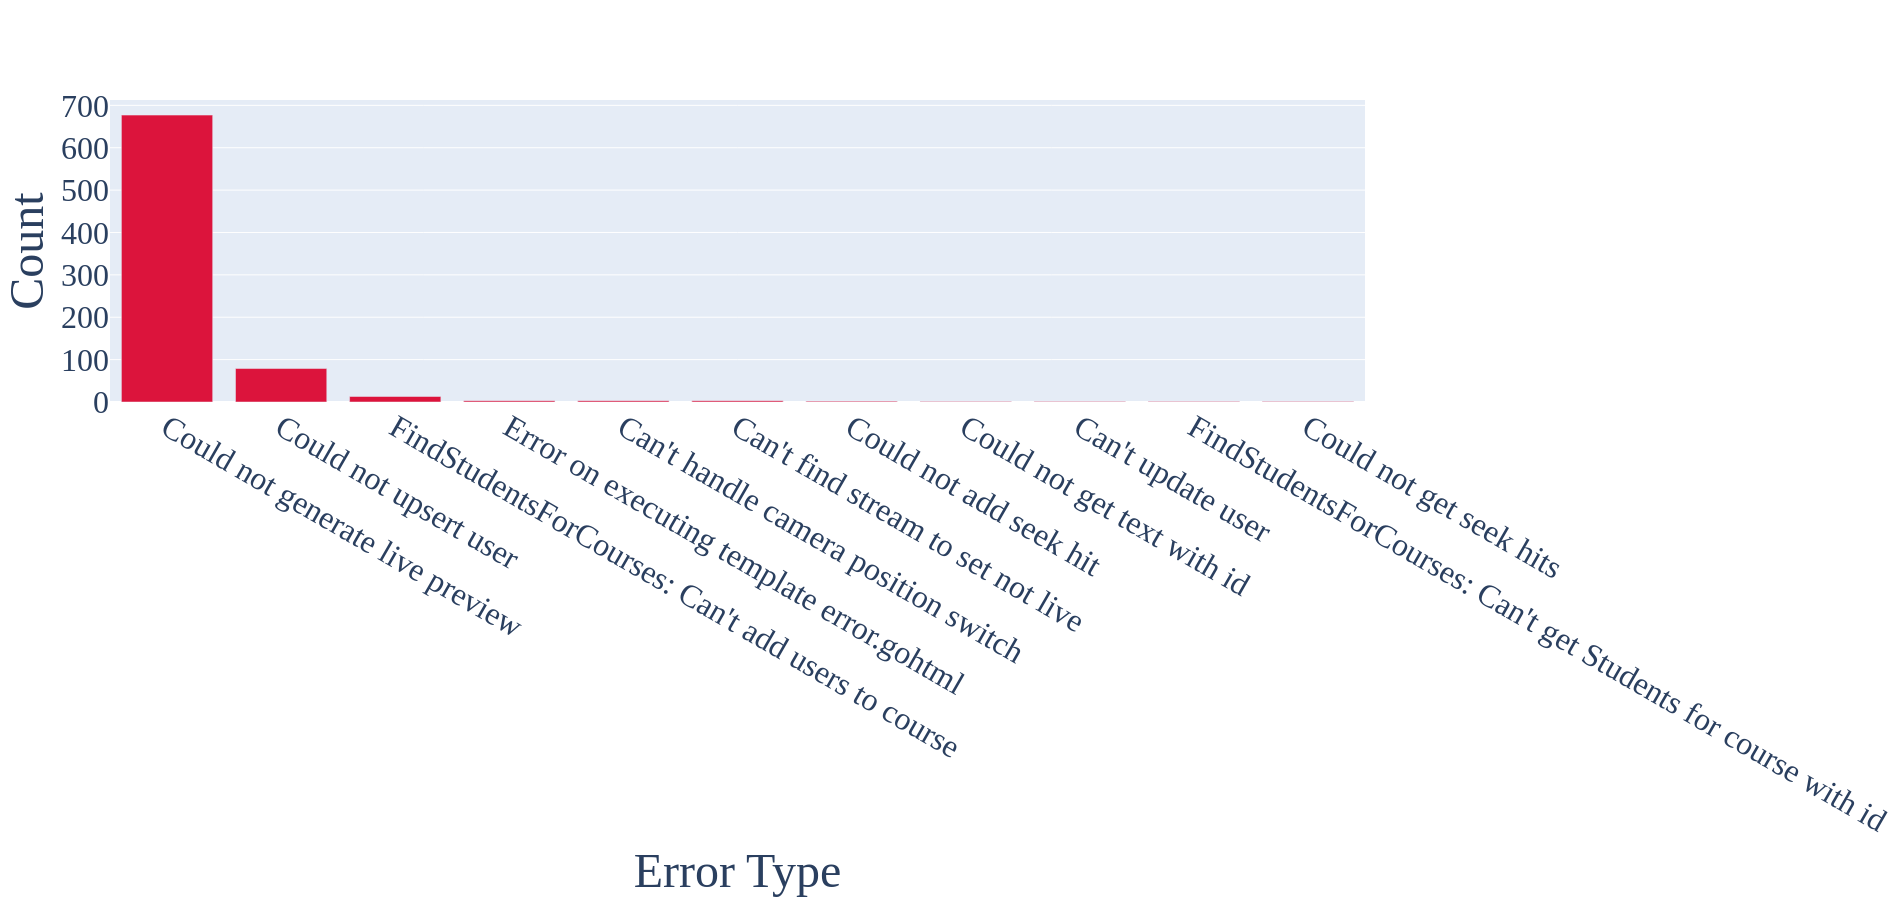
\includegraphics[width=\linewidth]{images/plots/api/error_types.png}
    \caption[\ac{API} Error Types]{\ac{API} Error Types}\label{fig:api-error-types}
\end{figure}

When aggregating the errors by their hour and plotting them in a bar chart grouped by error type (\autoref{fig:api-errors-by-hour-and-type}), there's an interesting observation that the \textit{'Could not generate live preview'} error, which is the most common error, mainly occurs during normal lecture times from 6AM. to 5PM. As the number of reported occurrences of this error is constant over these hours, it can be assumed that it is either an issue with an individual worker that might have a connection issue or is running an outdated docker image (the log data doesn't provide information on which \ac{VM} the error occurred), or a bug that affects all Workers. However, since we know that the \ac{API} fetches the previews once every minute from all Workers, and the number of errors per hour is around 60, it is most likely an issue with one individual Worker. If the issue was a random connection error, the number of occurrences should vary significantly and if the issue was a system-wide misconfiguration or bug in the Worker microservice, the error should occur on all Workers, meaning that the number of errors should be: \texttt{number of workers * 60}.     

\begin{figure}[htpb]
    \centering
    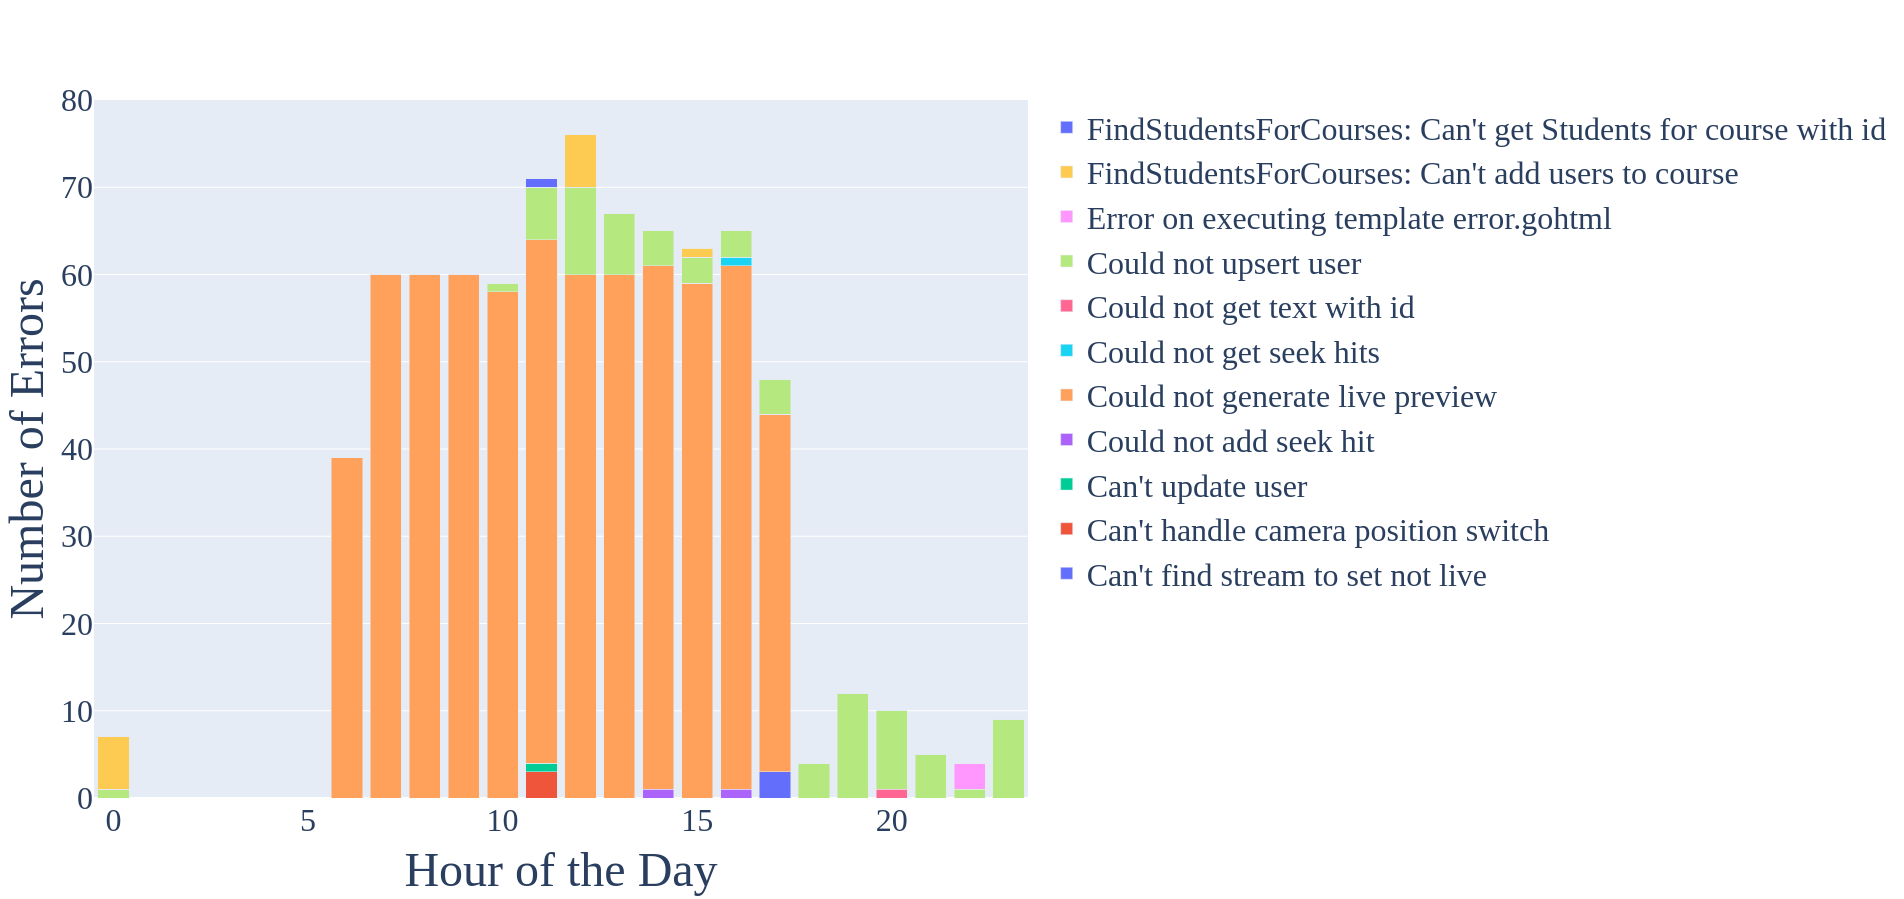
\includegraphics[width=\linewidth]{images/plots/api/errors_by_hour_and_type.png}
    \caption[\ac{API} Errors by Hour and Type]{\ac{API} Errors by Hour and Type}\label{fig:api-errors-by-hour-and-type}
\end{figure}

% \begin{figure}[htpb]
%     \centering
%     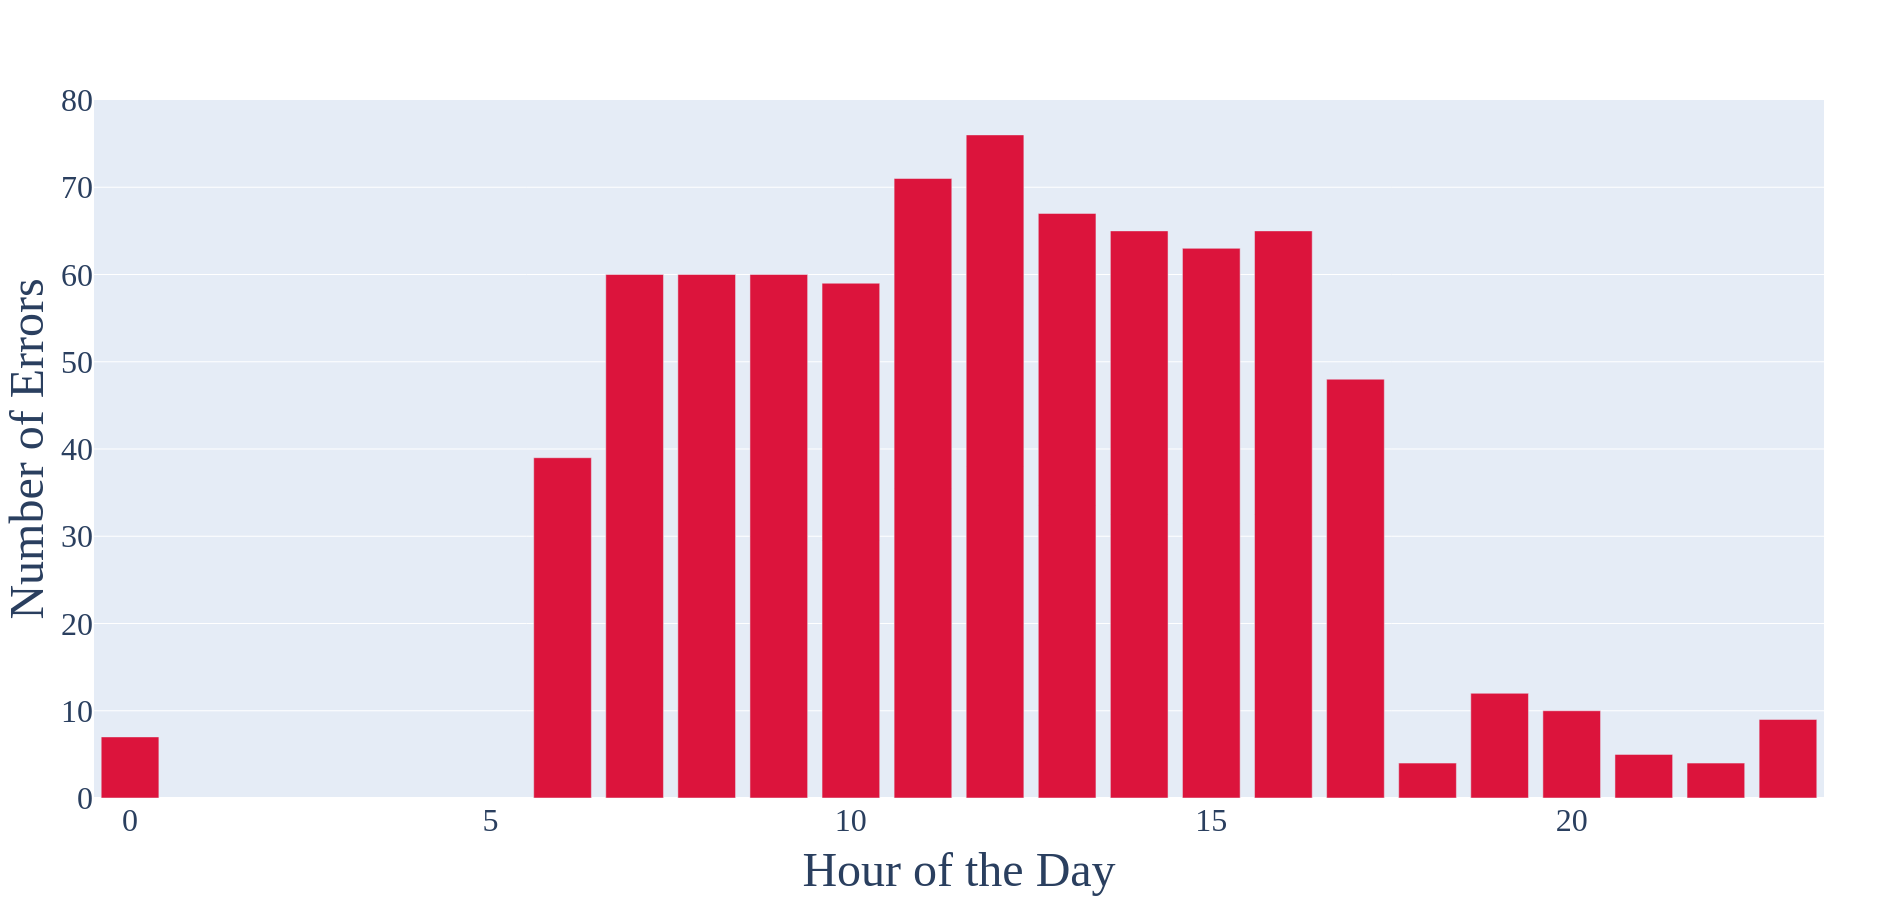
\includegraphics[width=\linewidth]{images/plots/api/errors_by_hour.png}
%     \caption[\ac{API} Errors by Hour]{\ac{API} Errors by Hour}\label{fig:api-errors-by-hour}
% \end{figure}

\section{Performance Bottleneck: Worker}

Again, using data collected from various logging services and exported via GoCast's Grafana dashboard, this section will give some insights on common errors of the Worker microservice.

\subsection{Errors over Time}

Similarly to the main \ac{API}, the Worker logs too show a constant number of errors over time (see \autoref{fig:worker-cum-errors-over-time}) indicating that there are either bugs or network issues that continue to occur and without being solved. With an average of approximately 30 Worker-related errors per day and days with as much as 75 logged errors (see \autoref{fig:worker-upscaled-error-logs} it shows that the Worker system can become a bottleneck in the future. Especially considering that - in contrast to the main \ac{API} - there is not just one Worker deployed, but rather a few dozens, meaning that the number of errors will increase proportionally to the number of Workers deployed. 

\begin{figure}[htpb]
    \centering
    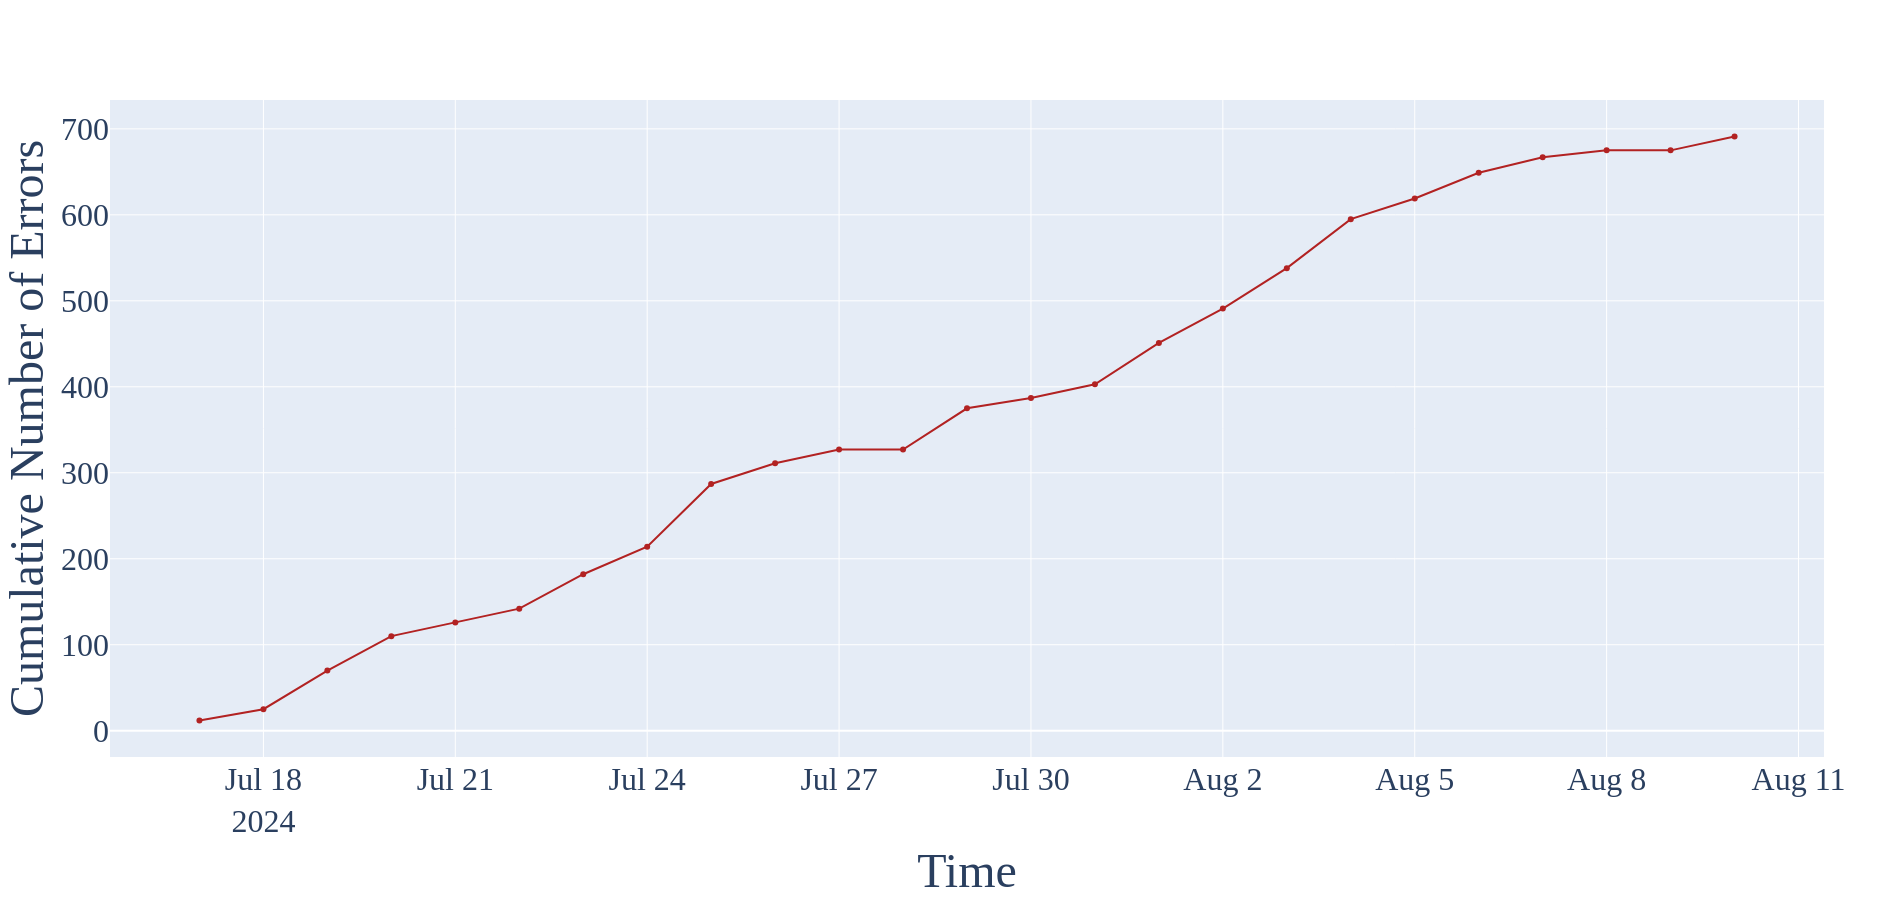
\includegraphics[width=\linewidth]{images/plots/worker/cum_errors_over_time.png}
    \caption[Cumulative Worker Errors Over Time]{Cumulative Worker Errors Over Time}\label{fig:worker-cum-errors-over-time}
\end{figure}

\begin{figure}[htpb]
    \centering
    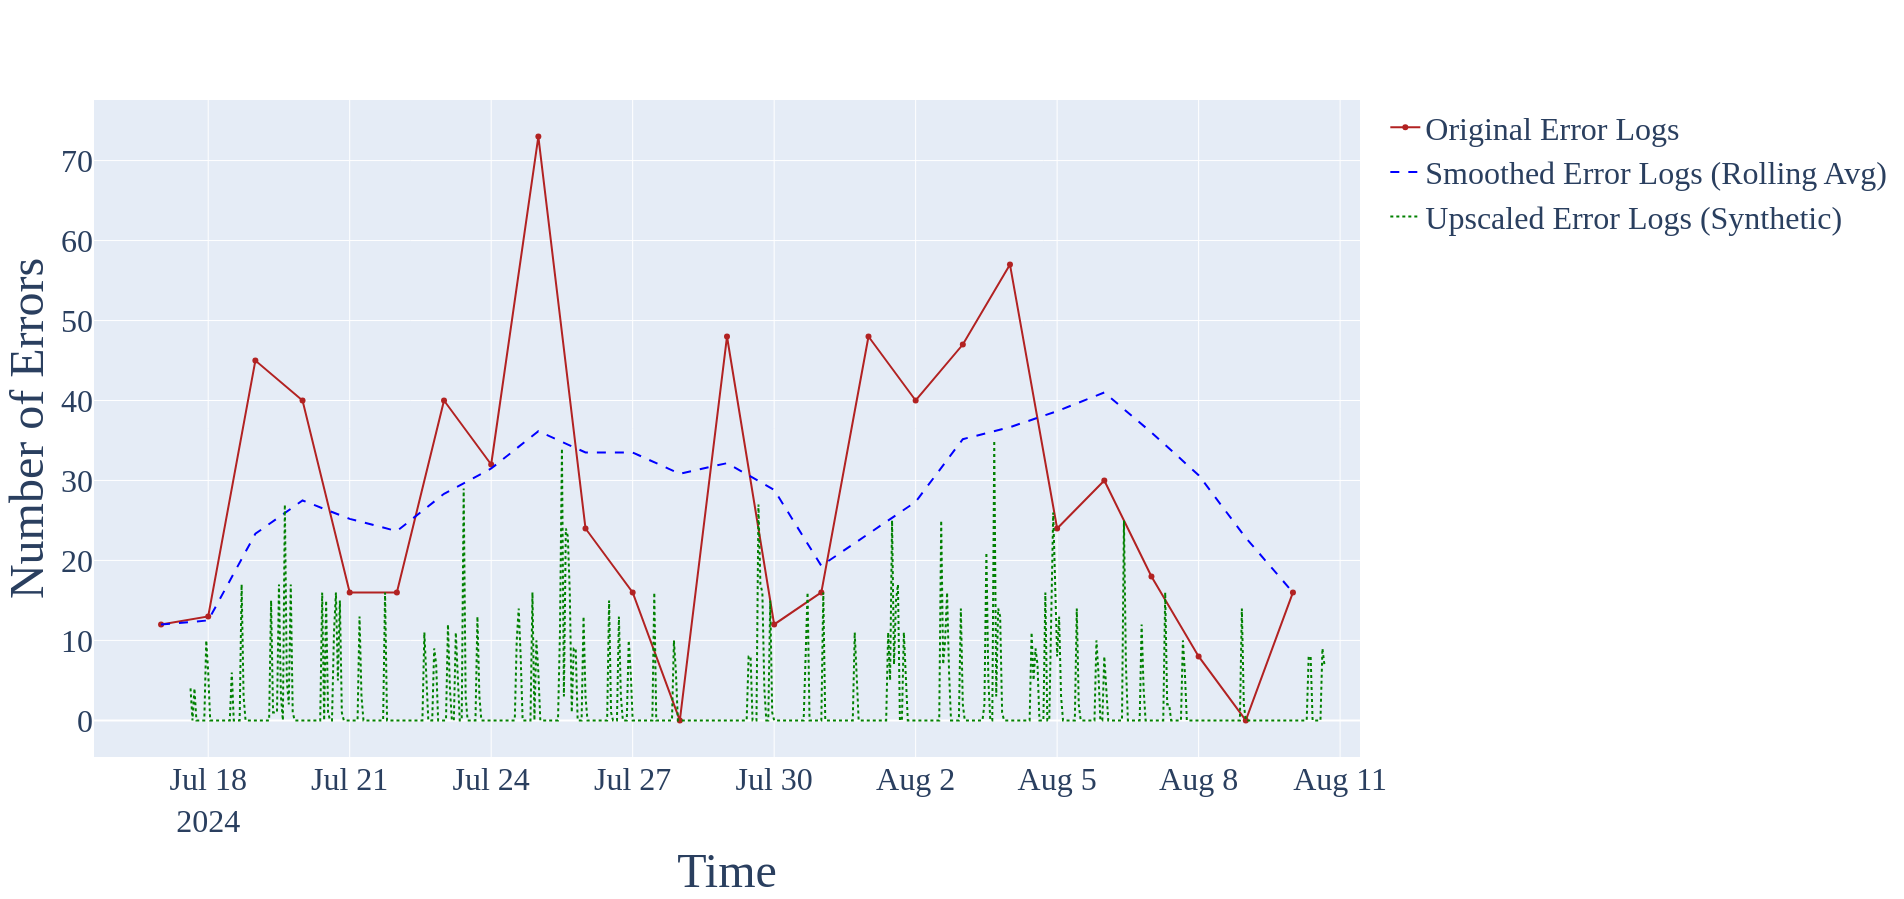
\includegraphics[width=\linewidth]{images/plots/worker/upscaled_error_logs.png}
    \caption[Upscaled Worker Error Logs]{Upscaled Worker Error Logs}\label{fig:worker-upscaled-error-logs}
\end{figure}

\subsection{The main Cause behind Worker Errors}

To find out what the main issue behind the Worker errors is, it is again helpful to take a look at the most common error types (see \autoref{fig:worker-error-types}. This shows that more than 90\% of the errors have the error log \textit{"Sending Heartbeat failed"}. A Worker sends once per minute a \textit{Heartbeat} HTTP request to the main \ac{API} with its current status and workload so that the \ac{API} has a current overview of all available workers and can decide which Workers to give tasks to. This error occurs however, when a Worker tries to send such a request and the request fails because the \ac{API} is unreachable. This can either occur because the \ac{API} has become unavailable or because the Worker's \ac{VM} has a network issue. As the main \ac{API} (besides two notable outages that lead to the API being offline for a few minutes) had an uptime of 99\%, the error is most likely with the Worker system itself. 

When taking a closer look at the actual logs, especially at other more critical error types that occur less often such as \textit{"Error uploading stream"}, it becomes clear that most of these errors are reported always by the two same Worker \ac{VM}s:

\begin{itemize}
    \item \texttt{labels=\{container=live\_worker..., error=Post "http://vodservice:8089": dial tcp 10.0.1.2:8089: i/o timeout, host=A, level=error, msg=Error\\ uploading stream, stream=..., time=...\}}

    \item \texttt{labels=\{container=live\_worker..., error=Post "http://vodservice:8089": dial tcp 10.0.1.2:8089: i/o timeout, host=B, level=error, msg=Error\\ uploading stream, stream=..., time=...\}}
\end{itemize}

Note that for simplicity, some information has been redacted from the logs and the hosts have been renamed to \texttt{A} and \texttt{B}. However, the main point remains that it appears that the errors occur due to a timeout when trying to reach the VOD Service. As all Workers run the same on the Worker-version and on similar \ac{VM}s, and only the two Workers on host \texttt{A} and \texttt{B} report timeout error, it might be due to a misconfiguration or separate issue with the \ac{VM} itself. 

\begin{figure}[htpb]
    \centering
    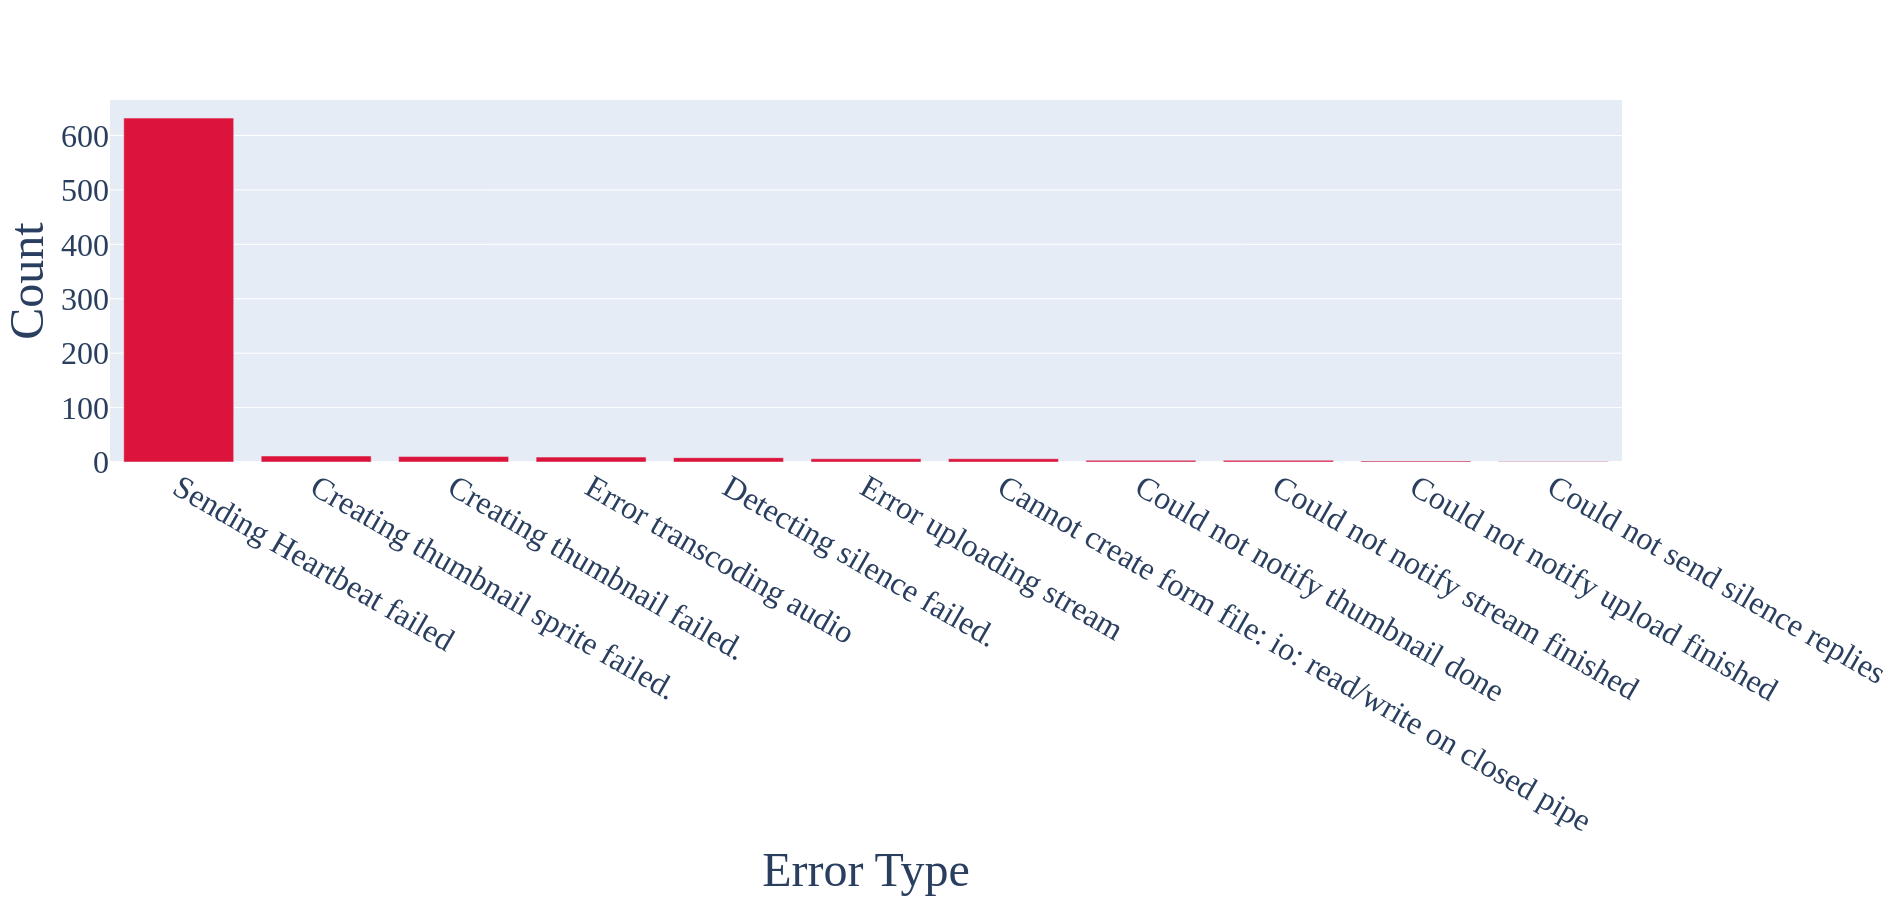
\includegraphics[width=\linewidth]{images/plots/worker/error_types.png}
    \caption[Worker Error Types]{Worker Error Types}\label{fig:worker-error-types}
\end{figure}

\subsection{Future Improvement: Runners}

At the time of this thesis, GoCast is developing a more robust and scalable alternative to the old Worker system: The Runner. In comparison to the Worker system, which receives a task (e.g., to upload a lecture) and then performs it straightaway, the Runner system works on the basis of queues and jobs. With this, incoming tasks are not just performed resulting in either success or an error, but rather scheduled and handled internally in such a way that a task consists of multiple jobs that can be prioritized accordingly, and, if failed, can be automatically retried multiple times before returning an error. Such a system would most likely solve errors such as the \textit{"Error uploading stream"} error mentioned before as the error would be handled internally and retried within certain time interval before reporting an error and aborting the task.

% \begin{figure}[htpb]
%     \centering
%     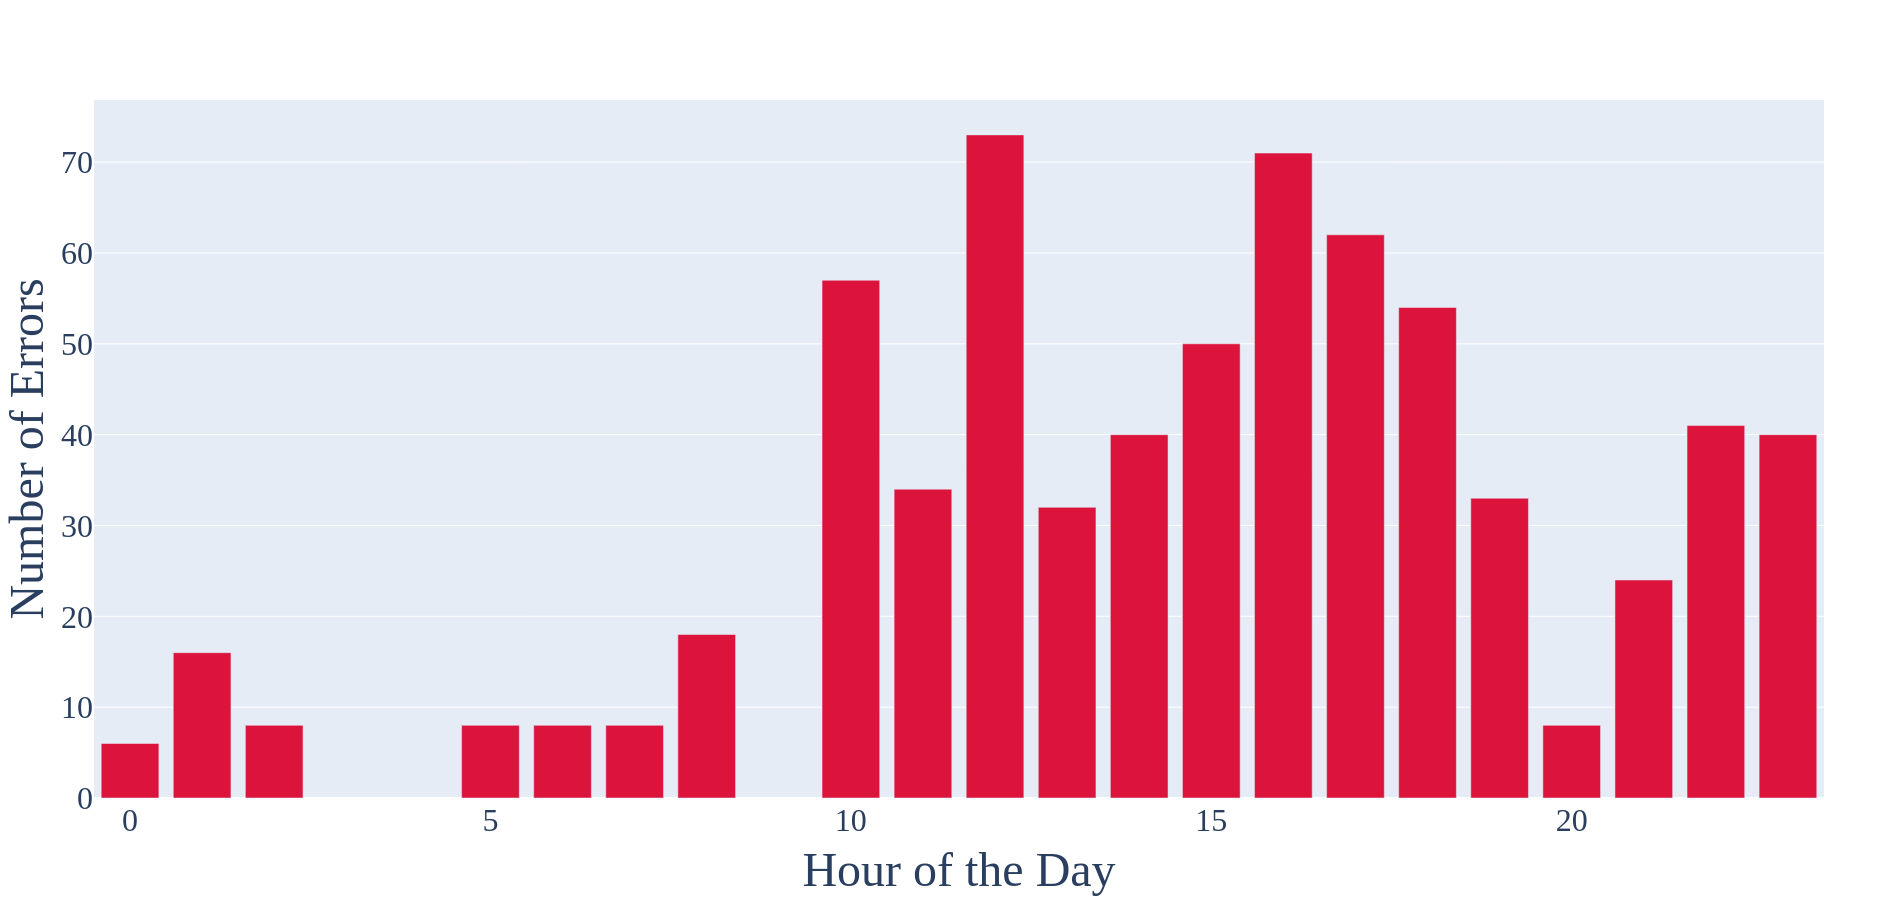
\includegraphics[width=\linewidth]{images/plots/worker/errors_by_hour.png}
%     \caption[Worker Errors by Hour]{Worker Errors by Hour}\label{fig:worker-errors-by-hour}
% \end{figure}

% Based on the collected metrics, the TUMLive Worker service was identified as a critical bottleneck. As the component responsible for encoding and uploading video streams, it often experiences high CPU and memory loads during peak usage times, leading to potential delays or errors.

% \section{Load Testing Edge Server and VOD Service}
% TODO

\section{A Technical Comparison of REST and gRPC APIs}

While analyzing the performance and limitations of the individual microservices of GoCast can help to resolve bottlenecks, at the core of the entire system there is still the main GoCast \ac{API}.
Most services (besides the VOD Service and Edge Servers) depend on the main \ac{API} to fetch up-to data information on streams and courses, to send updates on their current status and to notify it whenever there are new streams or \ac{VOD}s. Also, from the end-user's perspective, the API needs to be able to handle many concurrent requests as efficiently as possible to serve the actual streaming site and its data to the user's browser client.
Hence, in this section we'll focus on at two different \ac{API} design approaches: gRPC and REST.

\subsection{Why gRPC?}

gRPC, released in 2015 by Google, is a modern open-source high performance Remote Procedure Call (RPC) framework that can run cross-platform in any environment. It's strengths are that it can efficiently connect services, supports load balancing, tracing, health checking and authentication.
Another particularity of gRPC is that it automatically generate idiomatic client and server bindings for a service in a variety of languages and platforms using protofiles~\parencite{grpc_vs_rest}.
As it will become clear in the next subsections, it's main advantage over classical HTTP/REST \ac{API}s is that as is based on Protocol Buffers, it has a noticeable stronger performance~\parencite{grpc_vs_rest_2} and supports HTTP/2-based transport and bi-directional streaming, which is difficult with HTTP/1.1, and more efficient than using WebSockets for such purposes~\parencite{grpc_dev}.

\subsection{GoCast's gRPC Prototype and JMeter Test Setup}

GoCast's current REST API is written in Go using the \href{https://github.com/gin-gonic/gin}{Gin-Gonic} HTTP web framework. To test if a switch to gRPC would be useful, a prototype for a gRPC \ac{API} V2 was developed and can be found in the \href{https://github.com/carlobortolan/Thesis/tree/enh/api\_v2}{enh/api\_v2 branch of github.com/carlobortolan/Thesis}.
The prototype is based on the \href{https://google.golang.org/grpc}{official Go gRPC library} and uses \href{https://github.com/protocolbuffers/protobuf}{protoc} used to compile and generate Go code from the \texttt{.proto} files as well as \href{https://github.com/bufbuild/buf}{buf} for managing and generating protobuf files. Currently, only the most important original REST \ac{API} endpoints related to the user, course and stream management are supported by the prototype, as it is mainly intended for test purposes.

\subsubsection{JMeter Configuration and Data Collection}

To perform the performance tests that resulted in the data used in the following section, \href{https://jmeter.apache.org/}{Apache JMeter} - an open-source load tester and performance measurer was used. The main advantage of it is, that it exclusively works at protocol level, meaning that it appears and behaves like a browser (or rather, multiple browsers) to web-services, while not performing all the actions supported by browsers. The performed tests were structured using two thread groups - one for REST and one for gRPC - with each having three requests for the respective REST endpoints and gRPC methods:
\begin{itemize}
    \item REST: \texttt{GET:/courses}, \texttt{POST:/user/settings}, \texttt{PATCH:stream/bookmarks}
    \item gRPC: \texttt{getPublicCourses}, \texttt{postSettings}, \texttt{putBookmarks}
\end{itemize}
Each thread group used a thread pool (users) of size 150, a ramp-up period of 10 seconds and a repetition of 10.000 loops.
To measure, compare and export the response time, JMeter-listeners like \textit{Graph Results}, \textit{Summary Report} and \textit{Simple Data Writer} were used. To handle errors and check that the requests were performed successfully, JMeter’s \textit{View Results Tree} was used which captured any failed requests or error codes.

\subsection{Comparison of GoCast's gRPC Prototype and Current REST API}
The tests had a duration of 20 to 30 minutes and performed 1,196,180 HTTP requests with a mean response time of 644.55 ms and 1,171,342 gRPC requests with a mean response time of 162.69 ms. A more detailed overview can be found in \autoref{tab:rest_grpc_statistics}.

\begin{table}[htbp]
\centering
\caption{Statistical Analysis of REST and gRPC Data}
\label{tab:rest_grpc_statistics}
\begin{tabular}{|l|l|l|}
\hline
\textbf{Metric} & \textbf{REST API} & \textbf{gRPC API} \\ \hline
\textbf{Count} & 1,196,180 & 1,171,342 \\ \hline
\multicolumn{3}{|c|}{\textbf{Elapsed Time}} \\ \hline
Mean & 644.55 ms & 162.69 ms \\ \hline
Standard deviation & 60.38 ms & 36.13 ms \\ \hline
Min & 101 ms & 101 ms \\ \hline
25th percentile & 628 ms & 148 ms \\ \hline
Median (50th percentile) & 642 ms & 152 ms \\ \hline
75th percentile & 659 ms & 175 ms \\ \hline
Max & 4,562 ms & 2,090 ms \\ \hline
\multicolumn{3}{|c|}{\textbf{grpThreads (allThreads for REST)}} \\ \hline
Mean & 149.90 & 149.21 \\ \hline
Standard deviation & 2.94 & 2.28 \\ \hline
Min & 2 & 11 \\ \hline
25th percentile & 150 & 149 \\ \hline
Median (50th percentile) & 150 & 149 \\ \hline
75th percentile & 150 & 150 \\ \hline
Max & 150 & 150 \\ \hline
\end{tabular}
\end{table}

To evaluate whether gRPC provides significant enough benefits, the focus was on collecting and analyzing the following metrics:

\begin{itemize}
    \item 
        \textbf{Latency}: Response Time of an individual request - see \autoref{fig:comp-response-time} and \autoref{fig:comp-distribution}.
        \begin{figure}[htpb]
            \centering
                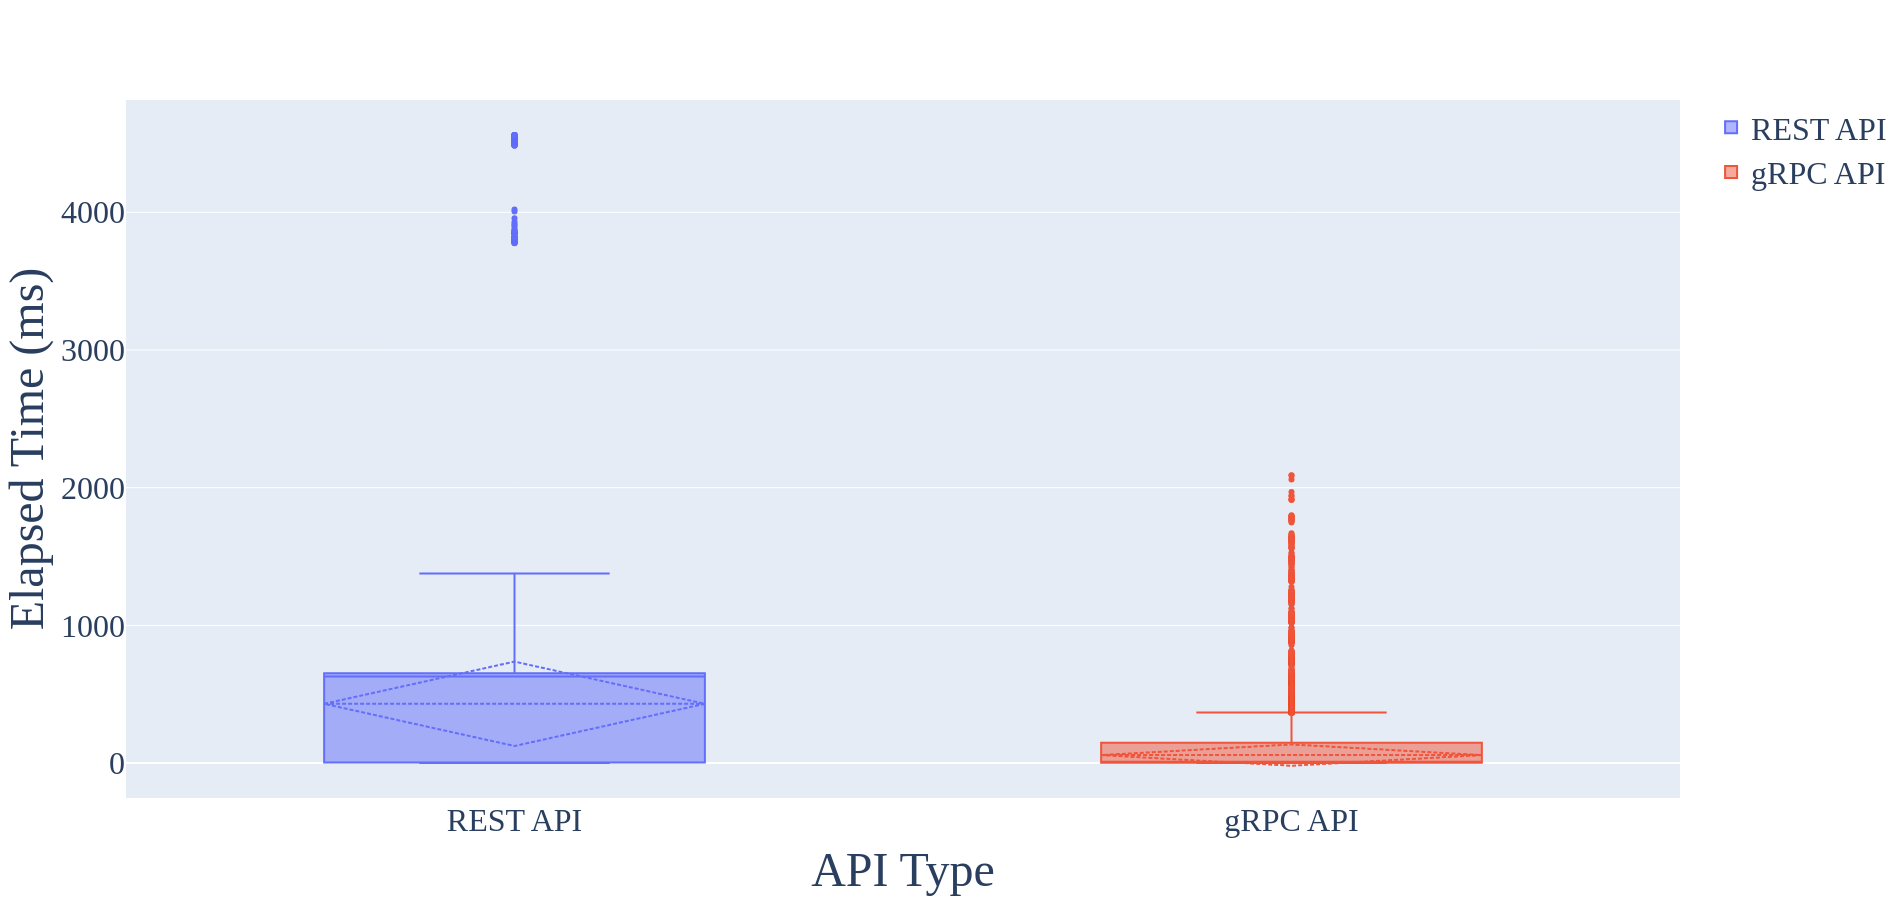
\includegraphics[width=\linewidth]{images/plots/comp/response_time_comparison.png}
            \caption[Response Time Comparison]{Response Time Comparison}\label{fig:comp-response-time}
        \end{figure}
        
        \begin{figure}[htpb]
            \centering
                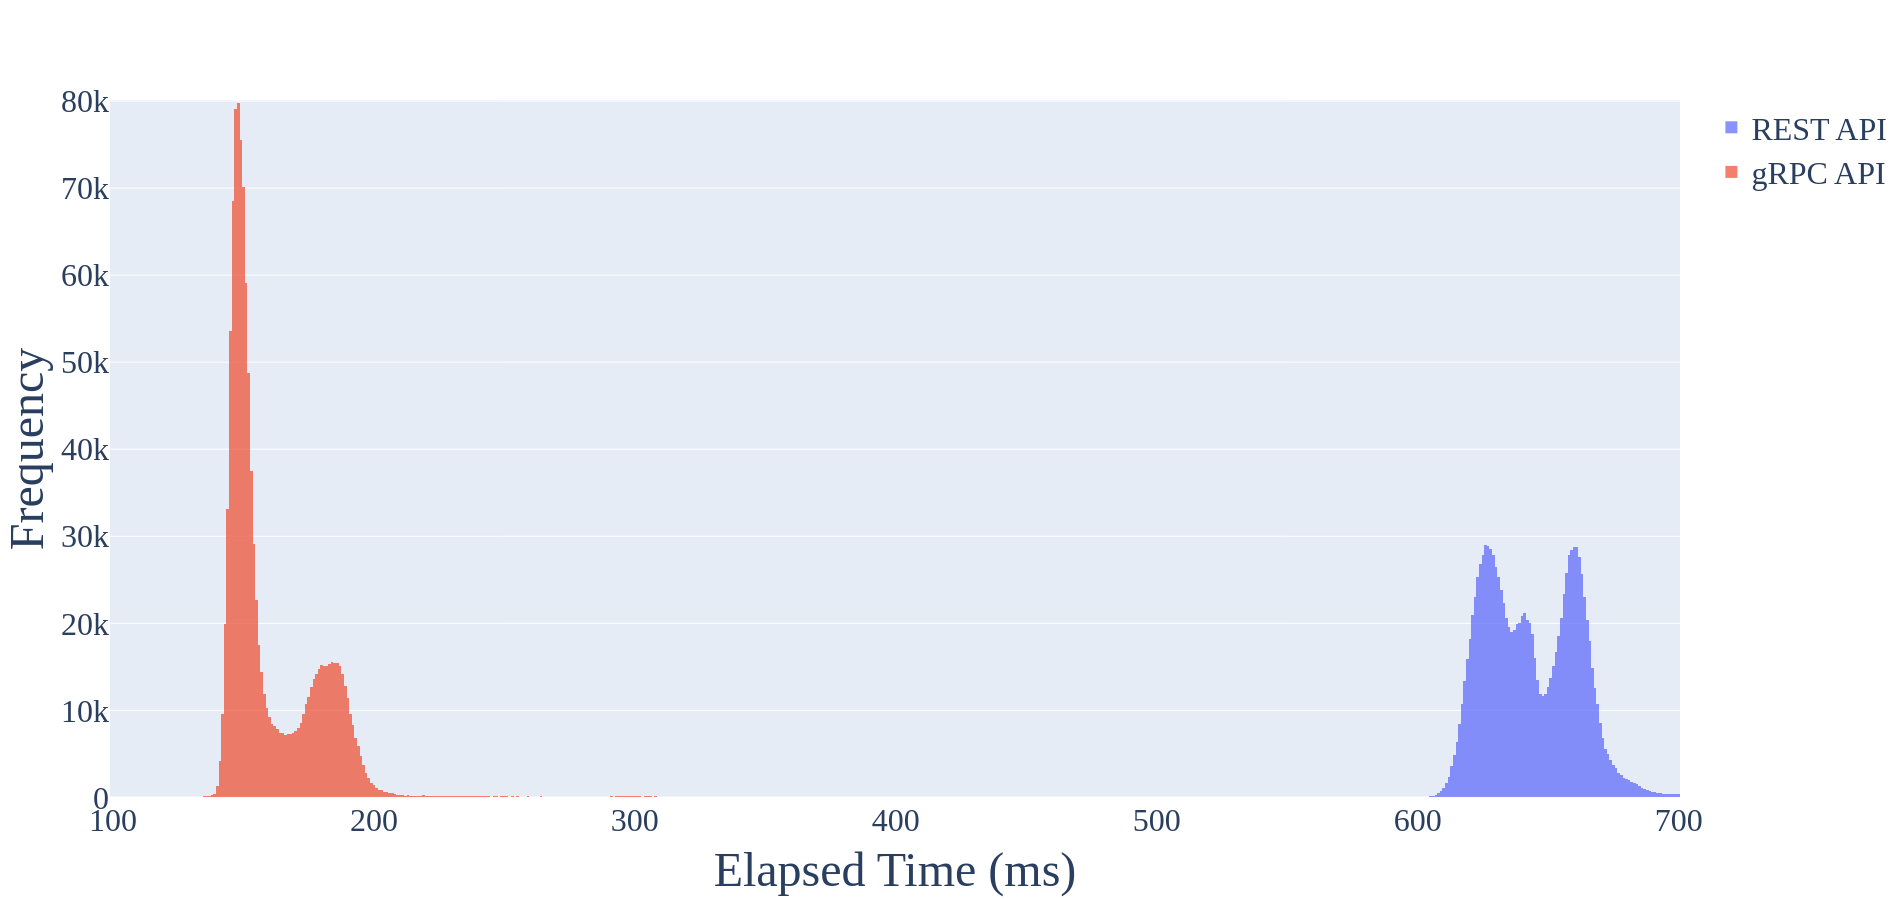
\includegraphics[width=\linewidth]{images/plots/comp/response_time_distribution.png}
            \caption[Response Time Distribution]{Response Time Distribution}\label{fig:comp-distribution}
        \end{figure}
    \item 
        \textbf{Throughput}: measures how many requests per minutes the \ac{API} can handle - see \autoref{fig:comp-throughput}
        \begin{figure}[htpb]
            \centering
                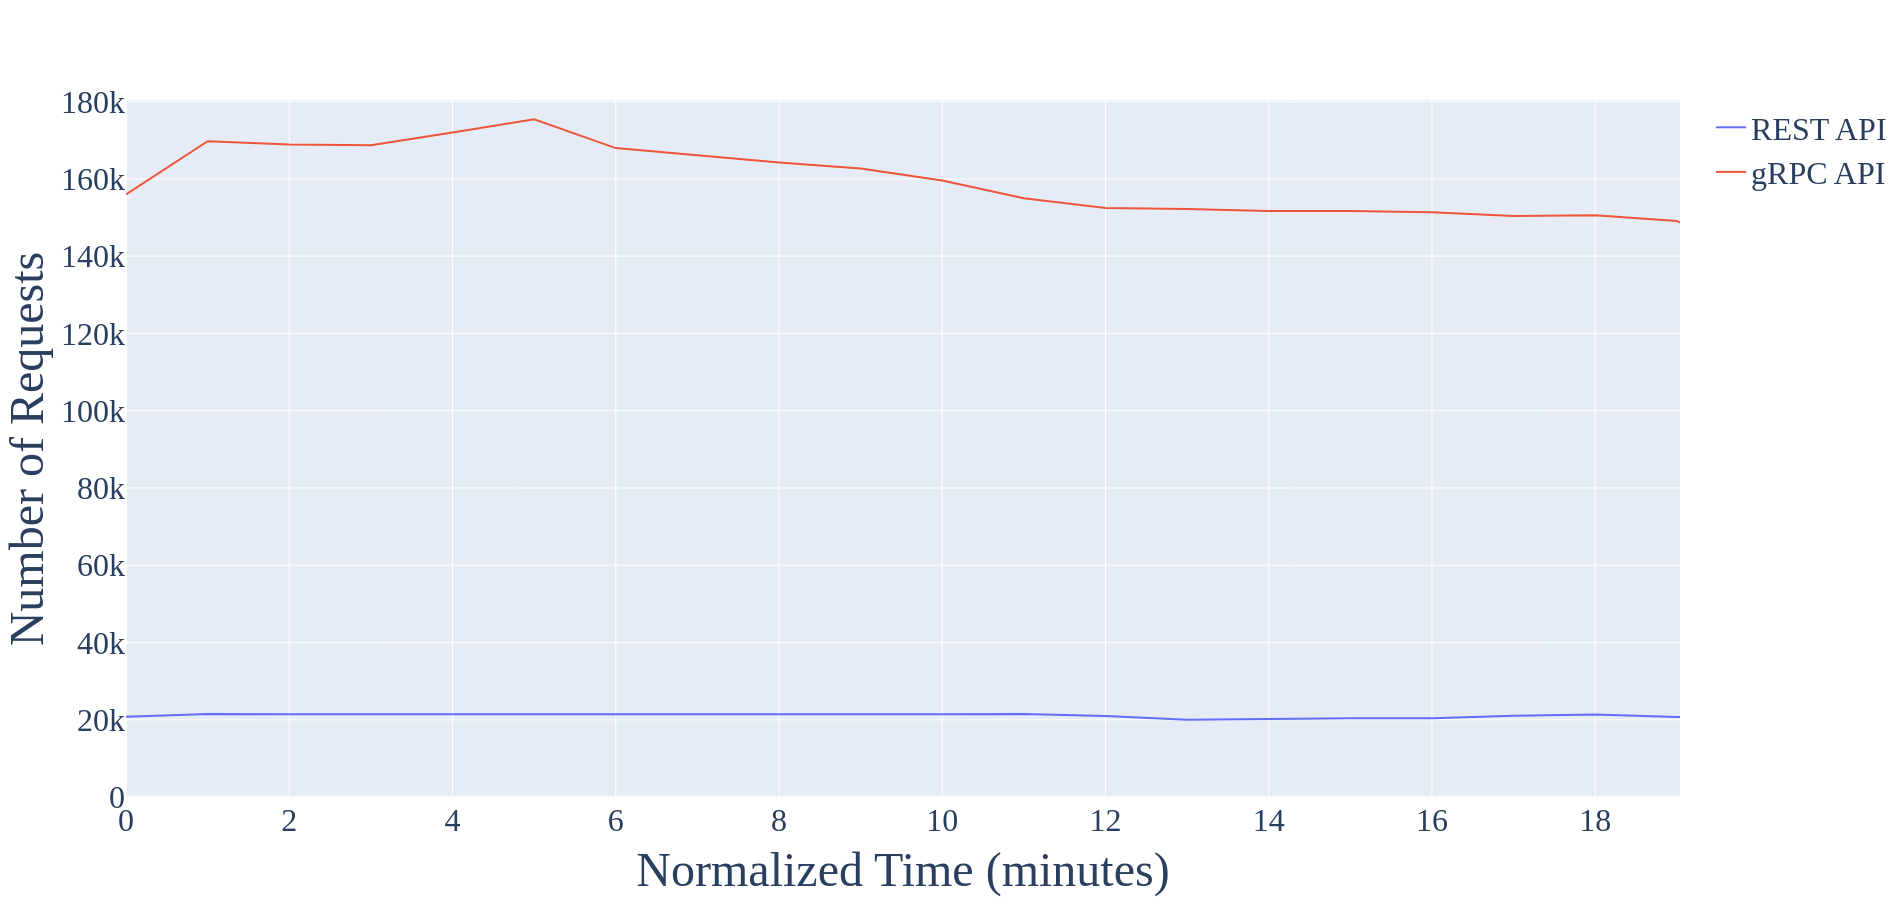
\includegraphics[width=\linewidth]{images/plots/comp/throughput_over_time.png}
            \caption[Throughput over Time]{Throughput over Time}\label{fig:comp-throughput}
        \end{figure}
\end{itemize}

\subsection{Results}

As expected, gRPC is significantly faster due to its use of Protocol Buffers and HTTP/2, which reduces overhead compared to HTTP/1.1. To evaluate whether gRPC justifies the effort of switching the API Design, there are three main considerations:

\begin{enumerate}
    \item \textbf{Performance Benefits}: gRPC offers approximately a 3-times significant reduction in latency and an 8 times increase in throughput. It can also be observed in \autoref{fig:comp-response-time} that the standard deviation of the response time with gRPC requests (36.13 ms) is nearly half that of HTTP requests (60.38 ms) which could lead to an overall more stable \ac{API} performance.  When considering outliers, the gRPC \ac{API} again outperforms the REST \ac{API}, having a maximum latency of 2,090 ms for slow requests compared to 4,562 ms for the REST \ac{API}.

    \item \textbf{Browser Compatibility}: While the lack of native browser support for gRPC might make REST a better fit, the current gRPC prototype exposes an HTTP Gateway that can be accessed just like a REST API by browser-based clients. Also, the gRPC prototype only contained "normal" endpoints, but considering the many real-time use cases that come with streaming (e.g., the live chat), gRPC’s bidirectional streaming could be a big advantage over REST.

    \item \textbf{Migration Effort}: Migrating to gRPC would require a complete re-implementation from scratch of the GoCast \ac{API} with significant changes clients and infrastructure. While tools for REST are widely spread (e.g., Postman, cURL), the gRPC ecosystem currently has fewer options for debugging, monitoring, and testing and often requires installing additional third-party add-ons to make commonly used tools compatible with gRPC. Also considering the time and resources needed for this transition, as well as experience of the developers that would have to work on this to handle gRPC and its related challenges, this might become an issue that outweighs the performance benefits.
\end{enumerate}

\section{Limitations of the Current System}

Given the analyzed data and review of GoCast's codebase, some limitations have been found that could become major issues when scaling up the current system.

\subsection{GoCast's In-Memory Chat System}

A major limitation of GoCast is its chat system. Currently, it is implemented as a combination of TCP and WebSockets to transmit real-time updates to viewers, but saves the actual chat channels in memory. This means that if the main API would be scaled to multiple instances and two users were to connect to two separate instances their chat messages would never reach the other instance. A possible solution for this problem would be to refactor the chat system on the server-side to store the chat messages in a separate in-memory database such as \href{https://redis.io/}{Redis} or use distributed messaging services such as \href{https://github.com/nats-io/nats-server}{NATS.io}. Alternatively, it is also possible to fix this issue by always having a certain GoCast instance being responsible for a certain chat or defining a hash function that determines depending on the current number of available instances, to which instance messages of a certain stream should be posted. 

\subsection{Other Factors for API Design}

While the gRPC prototype showed promising results, when it comes to comparing the different API design approaches, there are additional factors that can be considered:

\begin{itemize}
    \item \textbf{Resource Usage (CPU, Memory, Network)}
    It might be interesting to compare how efficiently each API handles resources under load. gRPC, with its smaller binary payloads, may consume less bandwidth, but may use more CPU. 
    Also, for potential bandwidth issues, network traffic could be analyzed to understand the differences in payload size and bandwidth usage.
    
    \item \textbf{Error Rates and Reliability}
    In a production-like environment it could be evaluated how both systems behave under load or failure scenarios. Does one API lead to more errors under heavy load, or can both handle the same level of traffic? One could measure the error rate (=percentage of failed requests during the test) or the time to recover from errors or failures (e.g., retries, handling transient errors, etc.).
\end{itemize}
